\section{Experimentos y evaluación}
\subsection*{Implementación del sistema}

\addtocounter{framenumber}{-1}
\begin{frame}[t]{Contenidos}{\textcolor{UniBlue}{.}}
	\tableofcontents[currentsection]
\end{frame}

\begin{frame}{Experimentos y evaluación}{Implementación del sistema}
\begin{itemize}
\item SPS S4 $\rightarrow$ Modifica el código fuente
	\begin{itemize}
		\item Cantidad de eventos entrantes y salientes de cada PE
	\end{itemize}
\item Distribución de la carga según la cola
	\begin{itemize}
		\item Política según el largo de la cola
	\end{itemize}
\end{itemize}

\begin{figure}
  \center
    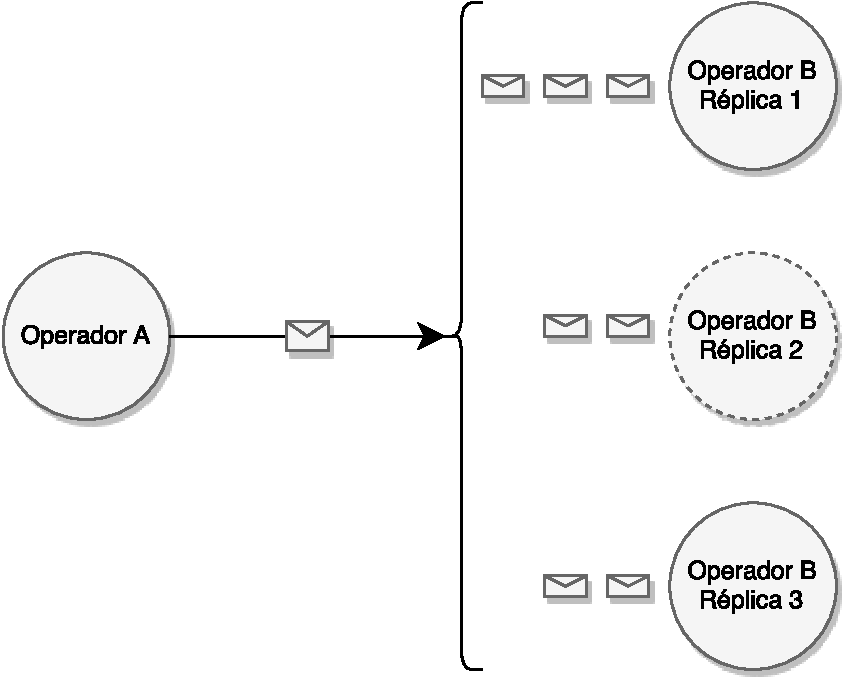
\includegraphics[scale=0.35]{images/DistribucionCarga-I.pdf}
\end{figure}
\end{frame}

\addtocounter{framenumber}{-1}
\begin{frame}{Experimentos y evaluación}{Implementación del sistema}
\begin{itemize}
\item SPS S4 $\rightarrow$ Modifica el código fuente
	\begin{itemize}
		\item Cantidad de eventos entrantes y salientes en cada PE
	\end{itemize}
\item Distribución de la carga según la cola
	\begin{itemize}
		\item Política según el largo de la cola
	\end{itemize}
\end{itemize}

\begin{figure}
  \center
    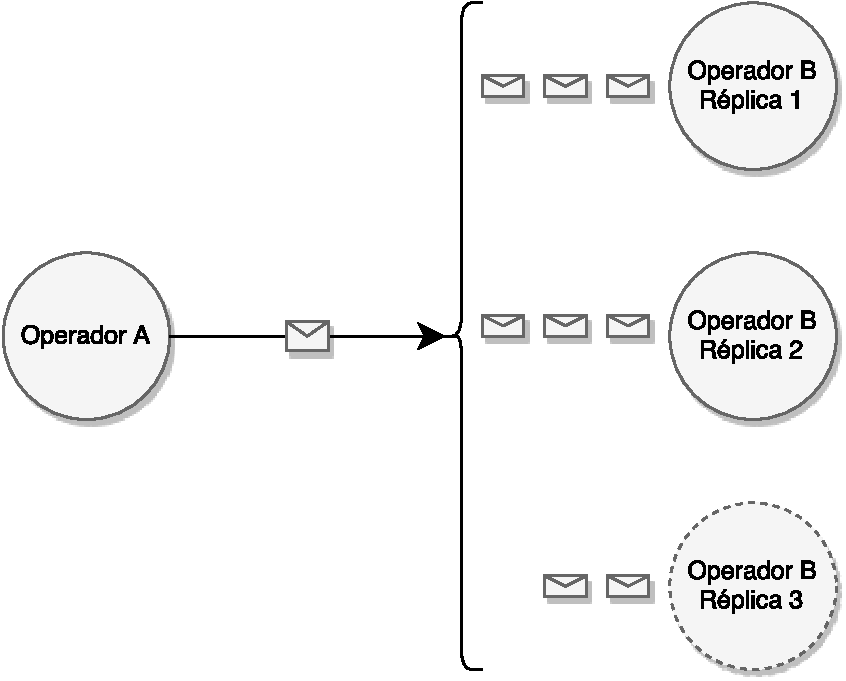
\includegraphics[scale=0.35]{images/DistribucionCarga-II.pdf}
\end{figure}
\end{frame}

\addtocounter{framenumber}{-1}
\begin{frame}{Experimentos y evaluación}{Implementación del sistema}
\begin{itemize}
\item SPS S4 $\rightarrow$ Modifica el código fuente
	\begin{itemize}
		\item Cantidad de eventos entrantes y salientes en cada PE
	\end{itemize}
\item Distribución de la carga según la cola
	\begin{itemize}
		\item Política según el largo de la cola
	\end{itemize}
\end{itemize}

\begin{figure}
  \center
    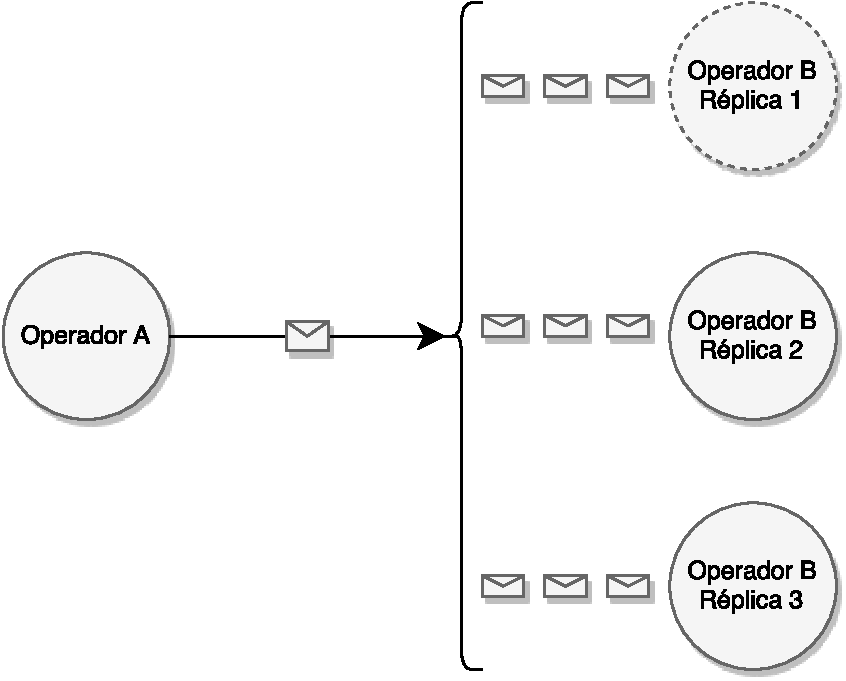
\includegraphics[scale=0.35]{images/DistribucionCarga-III.pdf}
\end{figure}
\end{frame}

\subsection*{Diseño de los experimentos}
\begin{frame}{Experimentos y evaluación}{Diseño de los experimentos}
\begin{itemize}
\item Dos tipo de aplicaciones
	\begin{itemize}
		\item Aplicación funcional
		\item Aplicación sintética
	\end{itemize}
\item Generación de stream
\begin{itemize}
	\item 4.5 millones de tweets
	\item 27-28 de Febrero y 1-2 de Marzo de 2010
	\item Inglés, español y portugués
	\item Interacción entre usuarios durante el terremoto del 27 de Febrero en Chile
\end{itemize}
\end{itemize}
\end{frame}

\begin{frame}{Experimentos y evaluación}{Diseño de los experimentos}
\begin{itemize}
	\item Aplicación funcional: Análisis de \textit{tweets} en escenarios de desastres naturales
	\begin{itemize}
		\item Validación del modelo dado un escenario aplicado
	\end{itemize}
\end{itemize}
\begin{figure}[!hb]
	\centering
		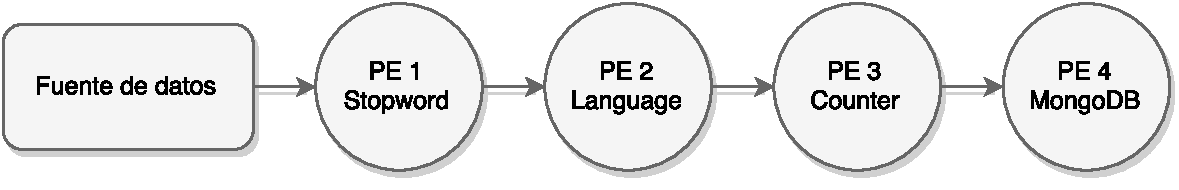
\includegraphics[scale=0.55]{images/App1.pdf}
\end{figure}
\end{frame}

\begin{frame}{Experimentos y evaluación}{Diseño de los experimentos}
\begin{itemize}
	\item Aplicación sintética
	\begin{itemize}
		\item Costos del uso del monitor
	\end{itemize}
\end{itemize}
\begin{figure}[!ht]
	\centering
		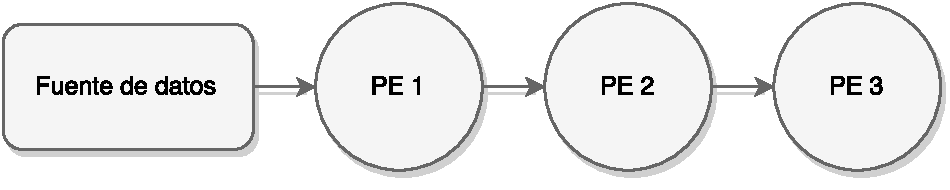
\includegraphics[scale=0.65]{images/App3.pdf}
\end{figure}
\begin{itemize}
	\item Período de tiempo que duerme la hebra asignada al PE
	\begin{itemize}
		\item Basadas del promedio de ejecución de operadores
	\end{itemize}
\end{itemize}
\begin{table}[!ht]
\footnotesize
\centering
\begin{tabular}{| c | c |}
\hline
PE & Tiempo (ms) \\ \hline
1 & 20 \\
2 & 30 \\
3 & 15 \\\hline
\end{tabular}
\end{table}
\end{frame}

\subsection*{Evaluación}
\begin{frame}{Experimentos y evaluación}{Evaluación}
\begin{itemize}
\item Para la ejecución de todos los experimentos se ha utilizado una máquina con un Intel Xeon CPU E5-2650 v2 de 2.60 GHz, 32 GB de RAM y SO Ubuntu 14.04.2 LTS

\item Para la evaluación de la primera aplicación se han realizado dos experimentos con distintos tiempos de ejecución:
\begin{itemize}
\item En el primer experimento es 60 minutos
\item Y en el segundo experimento es 10 minutos
\end{itemize}

\item Para la evaluación de la segunda aplicación se ha realizado un experimento
\begin{itemize}
	\item Envío constante de 100 eventos/s
	\item Tiempo de ejecución de 15 minutos
\end{itemize}

\item Cada uno de los experimentos se prueba con y sin modelo elástico

\end{itemize}
\end{frame}

%%% App 1 - Dynamic %%%

\begin{frame}{Experimentos y evaluación}{Aplicación funcional - Experimento 1 - Rendimiento y cantidad de réplicas}

\begin{itemize}
\item 96 eventos/segundo con uso del modelo \textit{vs} 16 eventos/segundo sin uso del modelo
\item Incremento de 5 veces más eventos/segundo
\end{itemize}

\begin{multicols}{2}
\begin{figure}[p]
	\centering
	{\scriptsize Con uso del modelo elástico\\}
	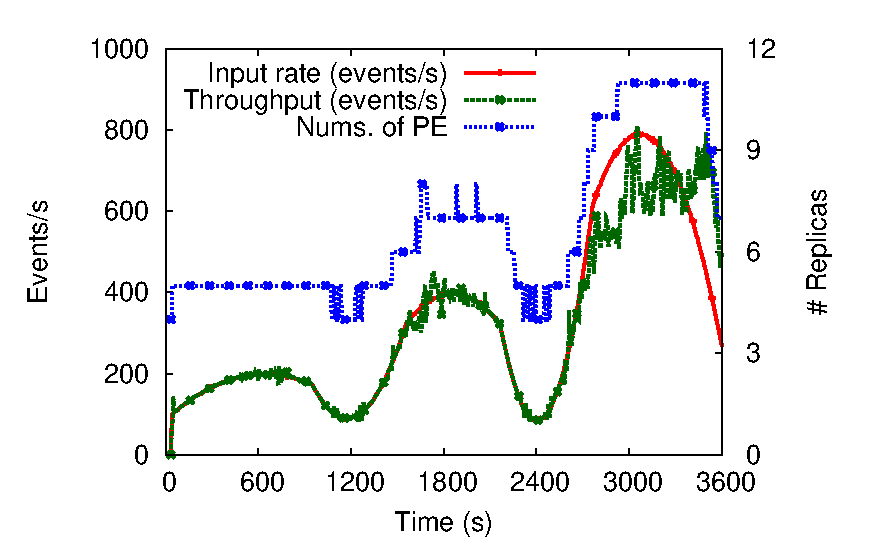
\includegraphics[scale=0.4]{images/exp/app1/dynamic/adaptative/exp1-processSystem.eps}
\end{figure}

\begin{figure}[p]
	\centering
	{\scriptsize Sin uso del modelo elástico\\}
	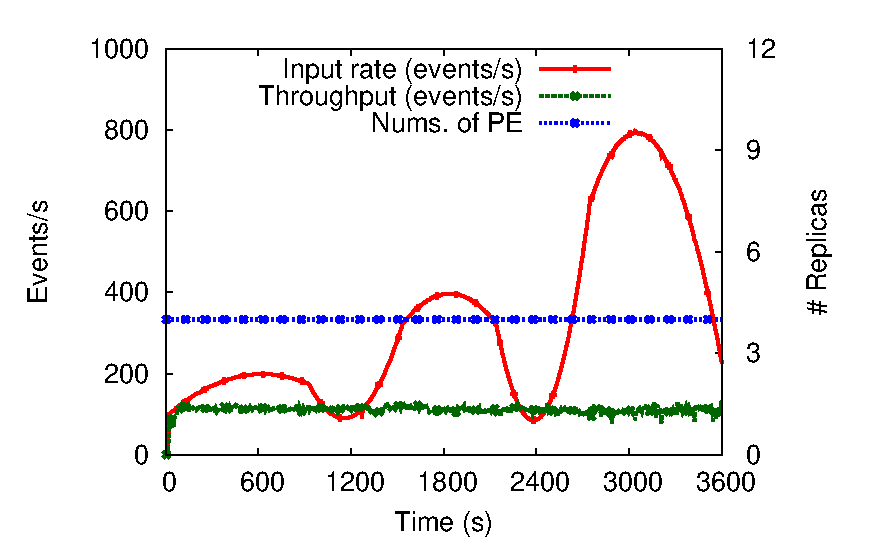
\includegraphics[scale=0.4]{images/exp/app1/dynamic/baseline/exp1-processSystem.eps}
\end{figure}
\end{multicols}
\end{frame}

\begin{frame}{Experimentos y evaluación}{Aplicación funcional - Experimento 1 - Cantidad total de eventos procesados}

\begin{itemize}
\item 1.139.537 eventos procesados con uso del modelo \textit{vs} 467.466 eventos procesados sin uso del modelo
\item Incremento de 2 veces la cantidad de eventos procesados
\end{itemize}

\begin{multicols}{2}
\begin{figure}[p]
	\centering
	{\scriptsize Con uso del modelo elástico\\}
	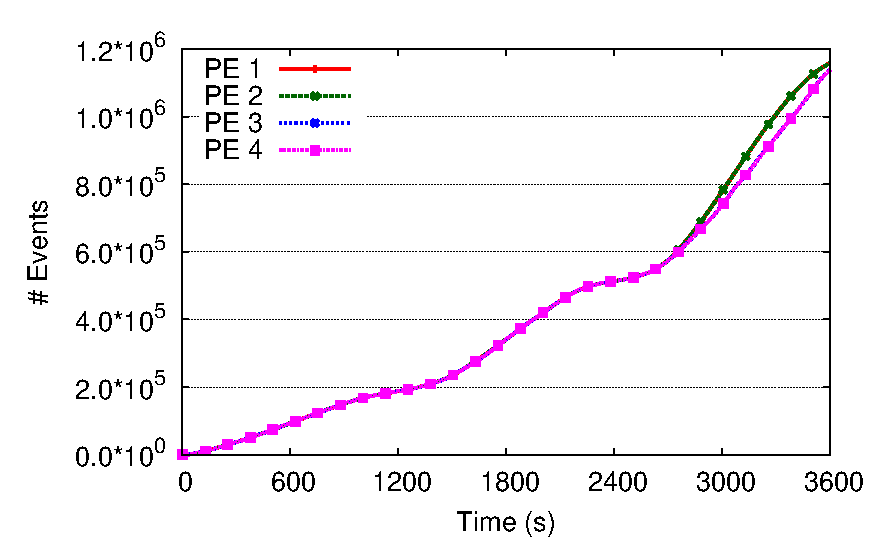
\includegraphics[scale=0.4]{images/exp/app1/dynamic/adaptative/exp1-eventCount.eps}
\end{figure}

\begin{figure}[p]
	\centering
	{\scriptsize Sin uso del modelo elástico\\}
	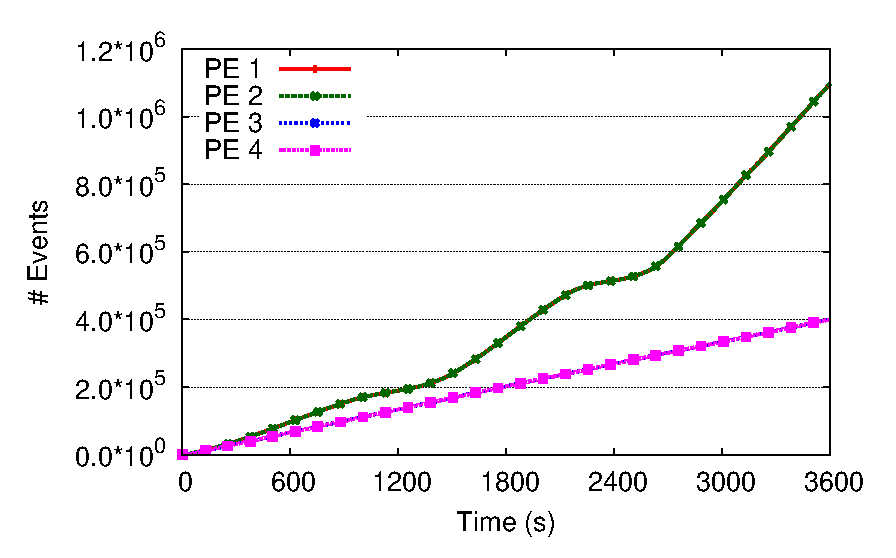
\includegraphics[scale=0.4]{images/exp/app1/dynamic/baseline/exp1-eventCount.eps}
\end{figure}
\end{multicols}
\end{frame}

%%% App 1 - Dynamic %%%
\begin{frame}{Experimentos y evaluación}{Aplicación funcional - Experimento 2 - Rendimiento y cantidad de réplicas}

\begin{itemize}
\item 72 eventos/segundo con uso del modelo \textit{vs} 19 eventos/segundo sin uso del modelo
\item Incremento de 3 veces más eventos/segundo
\end{itemize}

\begin{multicols}{2}
\begin{figure}[p]
	\centering
	{\scriptsize Con uso del modelo elástico\\}
	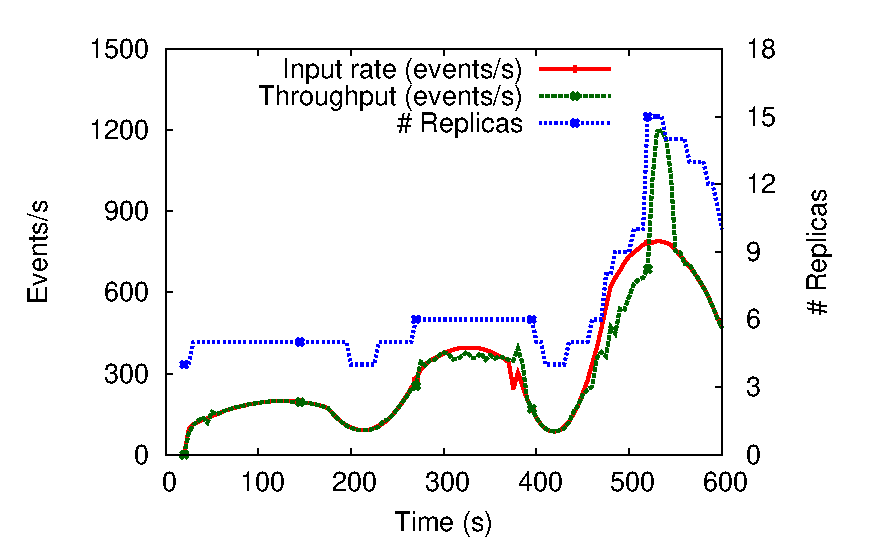
\includegraphics[scale=0.4]{images/exp/app1/dynamic/adaptative/exp2-processSystem.eps}
\end{figure}

\begin{figure}[p]
	\centering
	{\scriptsize Sin uso del modelo elástico\\}
	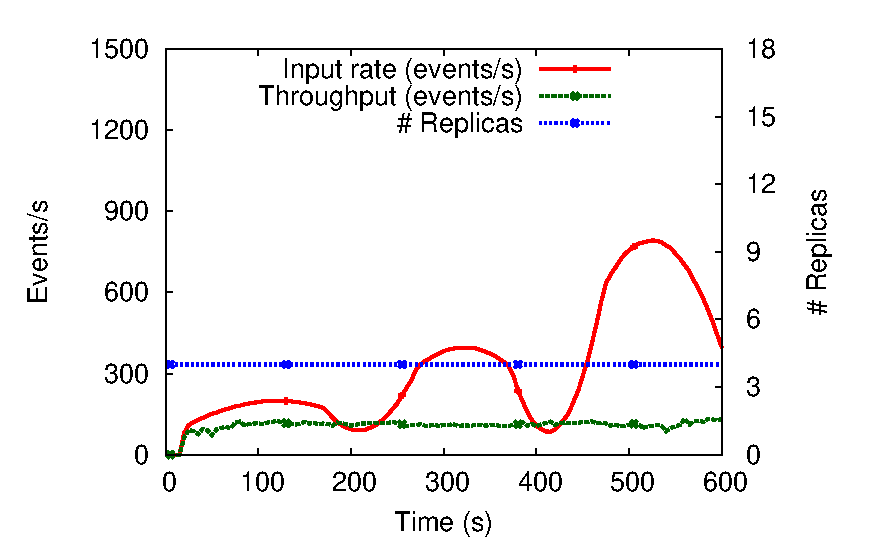
\includegraphics[scale=0.4]{images/exp/app1/dynamic/baseline/exp2-processSystem.eps}
\end{figure}
\end{multicols}
\end{frame}

\begin{frame}{Experimentos y evaluación}{Aplicación funcional - Experimento 2 - Cantidad total de eventos procesados}

\begin{itemize}
\item 201.751 eventos procesados con uso del modelo \textit{vs} 76.502 eventos procesados sin uso del modelo
\item Incremento de 2 veces la cantidad de eventos procesados
\end{itemize}

\begin{multicols}{2}
\begin{figure}[p]
	\centering
	{\scriptsize Con uso del modelo elástico\\}
	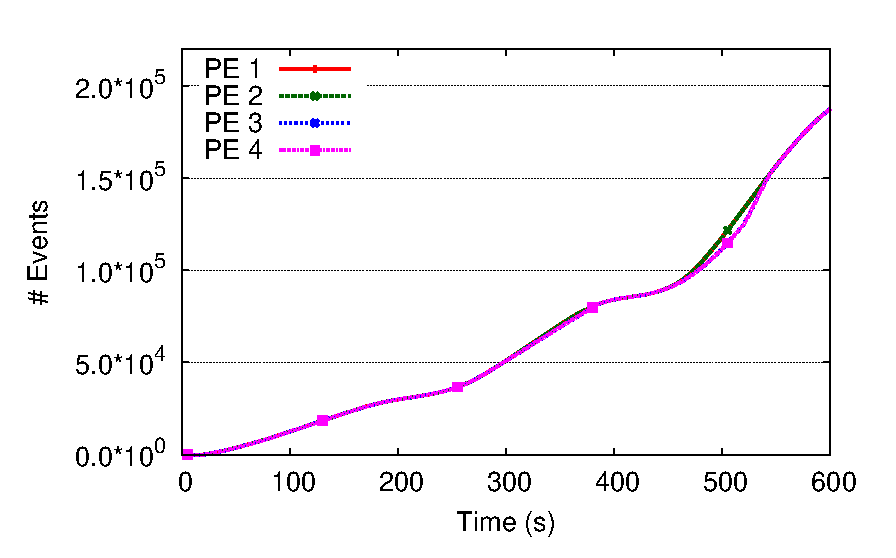
\includegraphics[scale=0.4]{images/exp/app1/dynamic/adaptative/exp2-eventCount.eps}
\end{figure}

\begin{figure}[p]
	\centering
	{\scriptsize Sin uso del modelo elástico\\}
	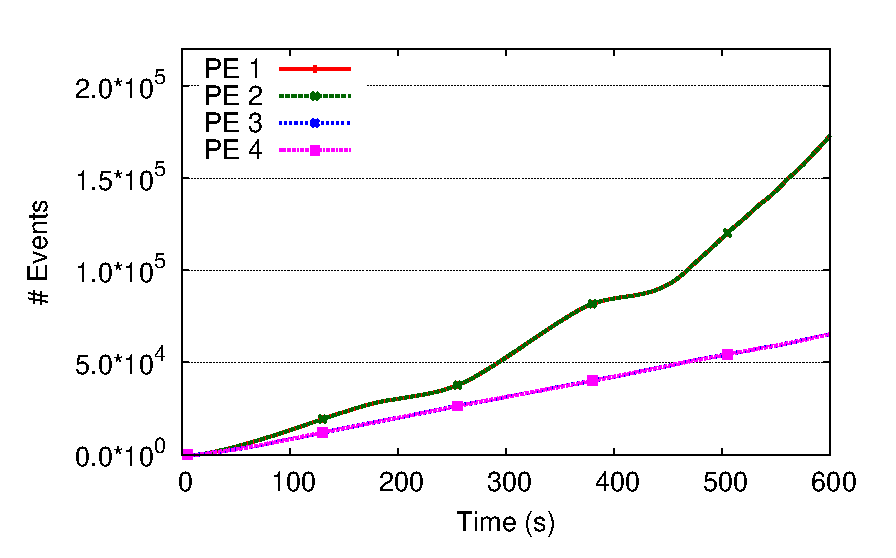
\includegraphics[scale=0.4]{images/exp/app1/dynamic/baseline/exp2-eventCount.eps}
\end{figure}
\end{multicols}
\end{frame}

%%% App 3 %%%

\begin{frame}{Experimentos y evaluación}{Aplicación sintética - Utilización promedio de CPU}

\begin{itemize}
\item $0,62\%$ promedio con uso del modelo \textit{vs} $0,61\%$ promedio sin uso del modelo
\item Aumento de un $0,01\%$ de utilización promedio de CPU
\end{itemize}

\begin{multicols}{2}
\begin{figure}[p]
	\centering
	{\scriptsize Con uso del modelo elástico\\}
	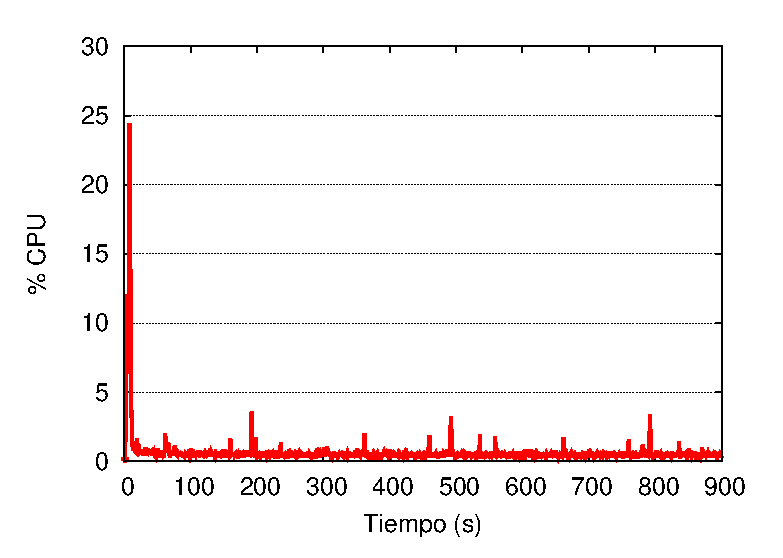
\includegraphics[scale=0.475]{images/exp/app3/cm/fisical/consumeCPU.eps}
\end{figure}

\begin{figure}[p]
	\centering
	{\scriptsize Sin uso del modelo elástico\\}
	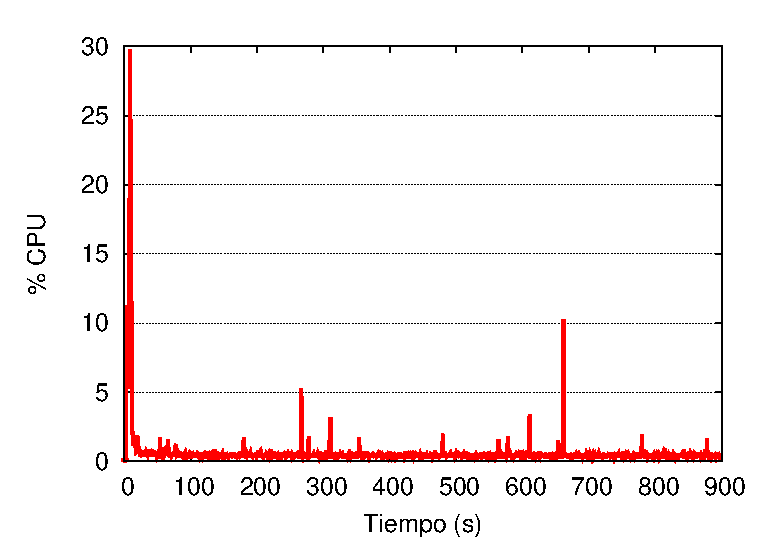
\includegraphics[scale=0.475]{images/exp/app3/sm/fisical/consumeCPU.eps}
\end{figure}
\end{multicols}
\end{frame}

\begin{frame}{Experimentos y evaluación}{Aplicación sintética - Consumo de memoria RAM}

\begin{itemize}
\item $264$MB con uso del modelo \textit{vs} $268$MB sin uso del modelo
\item Disminución de $1,5\%$ de consumo de memoria RAM
\end{itemize}

\begin{multicols}{2}
\begin{figure}[p]
	\centering
	{\scriptsize Con uso del modelo elástico\\}
	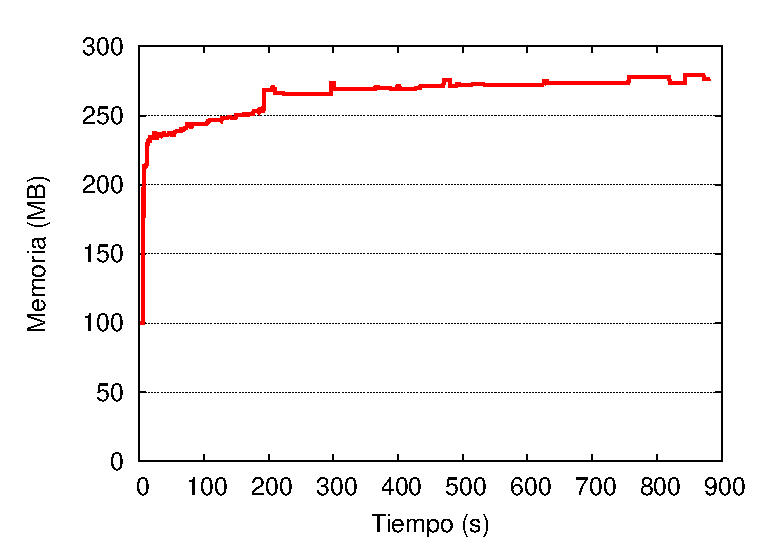
\includegraphics[scale=0.475]{images/exp/app3/cm/fisical/consumeRAM.eps}
\end{figure}

\begin{figure}[p]
	\centering
	{\scriptsize Sin uso del modelo elástico\\}
	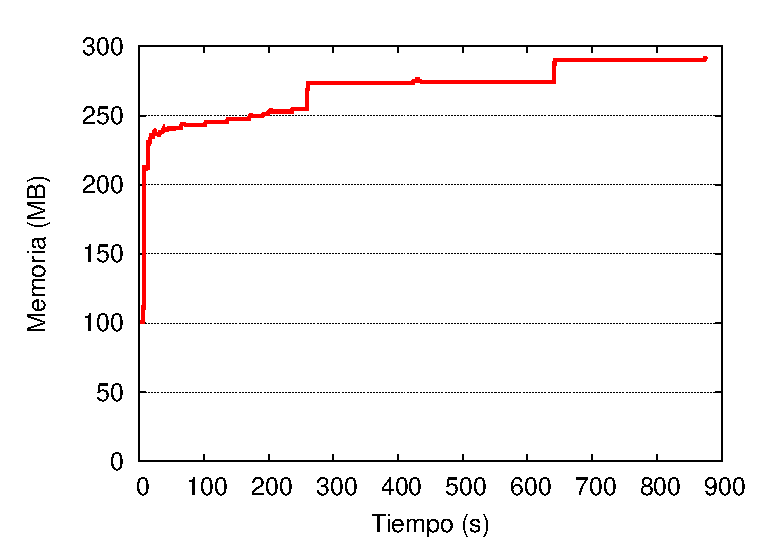
\includegraphics[scale=0.475]{images/exp/app3/sm/fisical/consumeRAM.eps}
\end{figure}
\end{multicols}
\end{frame}

\begin{frame}{Experimentos y evaluación}{Aplicación sintética - Tiempo de ejecución de cada algoritmo}
\begin{itemize}
	\item Algoritmo reactivo: 0.03 ms
	\item Algoritmo predictivo: 4.63 ms
\end{itemize}

\begin{figure}[p]
	\centering
	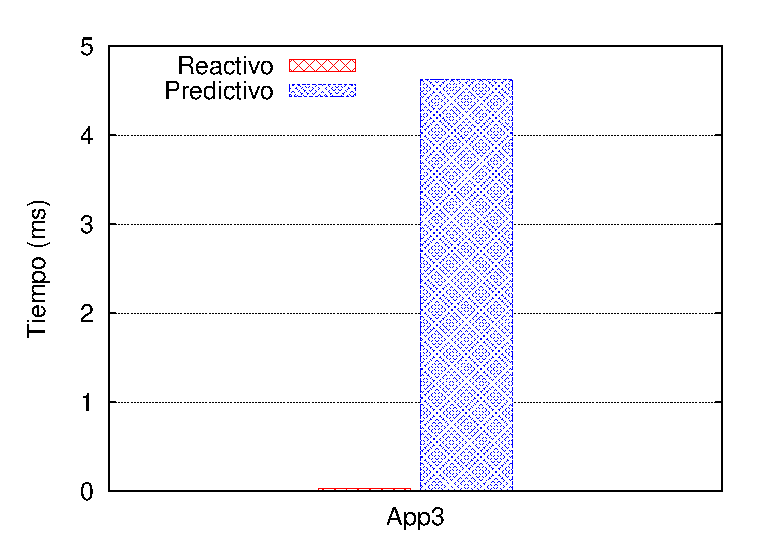
\includegraphics[scale=0.65]{images/exp/app3/cm/logical/tiempoAlgoritmos.eps}
\end{figure}

\end{frame}

\begin{frame}{Experimentos y evaluación}{Aplicación sintética - Rendimiento y cantidad de réplicas}

\begin{itemize}
\item 97 eventos/segundo con uso del modelo \textit{vs} 33 eventos/segundo sin uso del modelo
\item Incremento de 2 veces más eventos/segundo
\end{itemize}

\begin{multicols}{2}
\begin{figure}[p]
	\centering
	{\scriptsize Con uso del modelo elástico\\}
	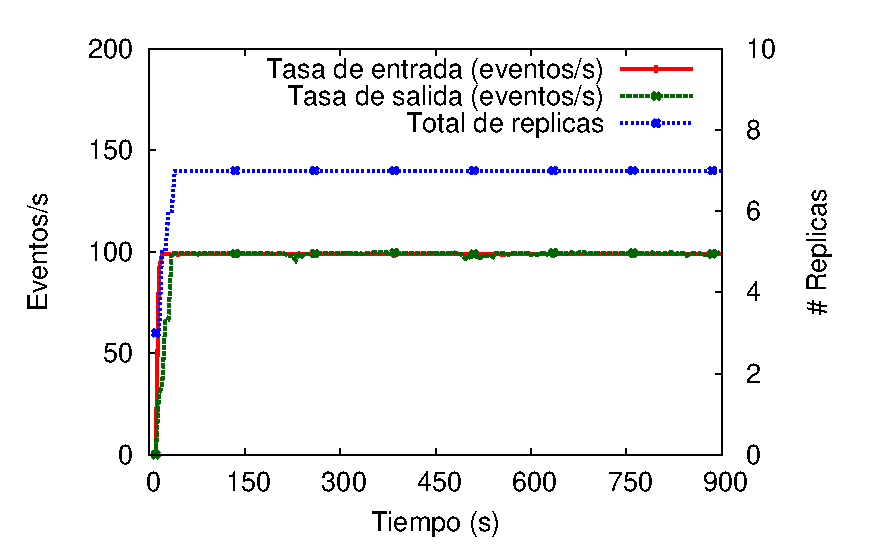
\includegraphics[scale=0.4]{images/exp/app3/cm/logical/processSystem.eps}
\end{figure}

\begin{figure}[p]
	\centering
	{\scriptsize Sin uso del modelo elástico\\}
	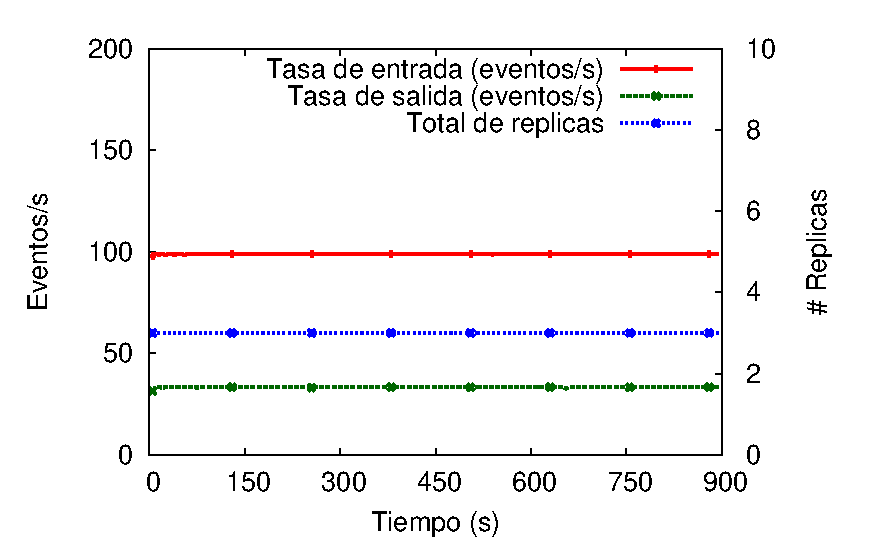
\includegraphics[scale=0.4]{images/exp/app3/sm/logical/processSystem.eps}
\end{figure}
\end{multicols}
\end{frame}

\begin{frame}{Experimentos y evaluación}{Aplicación sintética - Cantidad total de eventos procesados}

\begin{itemize}
\item 88.169 eventos procesados con uso del modelo \textit{vs} 28.714 eventos procesados sin uso del modelo
\item Incremento de 3 veces la cantidad de eventos procesados
\end{itemize}

\begin{multicols}{2}
\begin{figure}[p]
	\centering
	{\scriptsize Con uso del modelo elástico\\}
	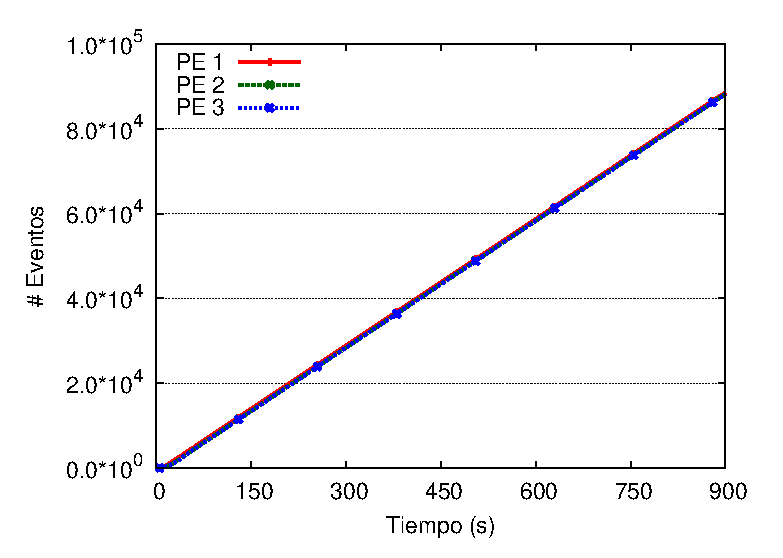
\includegraphics[scale=0.475]{images/exp/app3/cm/logical/eventCount.eps}
\end{figure}

\begin{figure}[p]
	\centering
	{\scriptsize Sin uso del modelo elástico\\}
	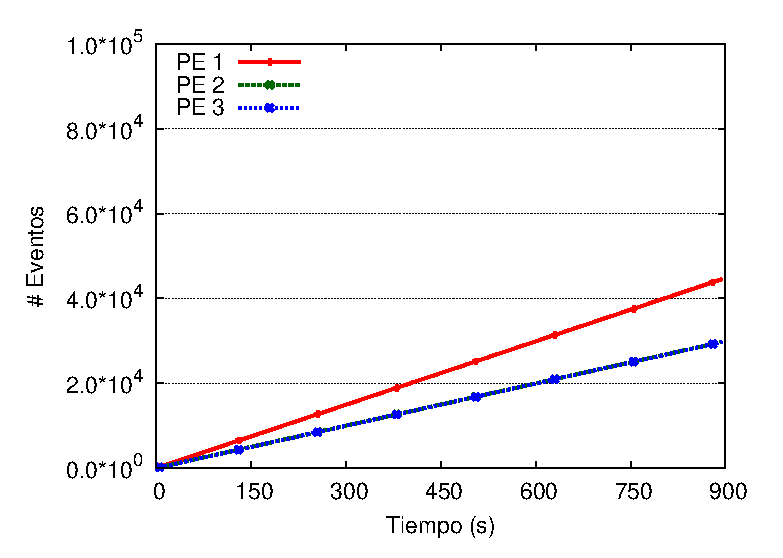
\includegraphics[scale=0.475]{images/exp/app3/sm/logical/eventCount.eps}
\end{figure}
\end{multicols}
\end{frame}